\section{Anforderungsanalyse}

\section*{2 Vorlesung 02}
\section*{2.1 wichtigste Begriffe des Usability-Engineering}
\begin{center}
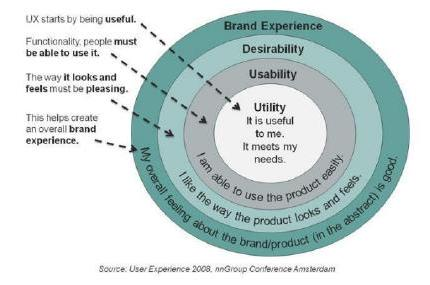
\includegraphics[max width=\textwidth]{2024_12_29_0d1d7b5551ea1b4b41bdg-02}
\end{center}

\begin{displayquote}
Abbildung 4: Usability und User Experience (UX)
\end{displayquote}

Usability = Deutsch: Gebrauchstauglichkeit\\
User Experience = Usability + Desirability\\
Customer Experience $=$ Usability + Desirability + Brand Experience

\subsection*{2.2 Usability-Anforderungen}
Die Effektivität, Effizienz und Zufriedenheit mit der die adressierten Benutzer ihre Ziele erreichen in ihren spezifischen Kontexten.

\section*{Wichtigste Aspekte}
\begin{itemize}
  \item Benutzer
  \item Seine Ziele/Aufgaben
  \item Sein Kontext
  \item Softwaresystem (inkl. UI)
\end{itemize}

\section*{Effektivität}
\begin{itemize}
  \item Der Benutzer kann alle seine Aufgaben vollständig erfüllen
  \item Mit der gewünschten Genauigkeit
\end{itemize}

Effizienz Der Benutzer kann seine Aufgaben mit minimalem/angemessenem Aufwand erledigen

\begin{itemize}
  \item Mental
  \item Physisch
  \item Zeit
\end{itemize}

\section*{Zufriedenheit Mit dem System / der Interaktion}
\begin{itemize}
  \item Minimum: Benutzer ist nicht verärgert
  \item Normal: Benutzer ist zufrieden
  \item Optimal: Benutzer ist erfreut
\end{itemize}

\subsection*{2.2.1 7 wichtige Anforderungsbereiche bezüglich Usability}
\begin{itemize}
  \item Aufgabenangemessenheit
  \item Lernförderlichkeit
  \item Individualisierbarkeit
  \item Erwartungskonformität
  \item Selbstbeschreibungsfähigkeit
  \item Steuerbarkeit
  \item Fehlertoleranz
\end{itemize}

\subsection*{2.3 User-Centered Designs}
\begin{center}
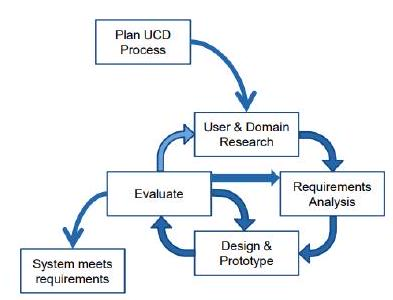
\includegraphics[max width=\textwidth]{2024_12_29_0d1d7b5551ea1b4b41bdg-03}
\end{center}

Abbildung 5: Usercentered Design

\subsection*{2.4 Ziele, Methoden und Artefakte der einzelnen Phasen des UCD}
\begin{itemize}
  \item Personas (Fiktive Person mit Eigenschaften / Fähigkeiten): Repräsentitert eine bestimmte Benutzergruppe
  \item Usage-Szenarien
  \item Mentales Modell
  \item Domänenmodell
  \item Service Blueprint / Geschäftsprozessmodell: Skizze wie Funktioniert was im Geschäft und was für Interaktionen geschehen wo
  \item Stakeholder Map\\
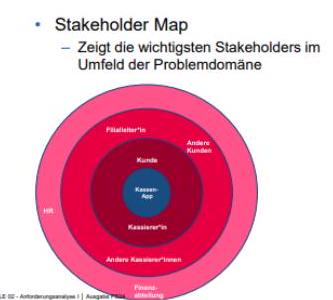
\includegraphics[max width=\textwidth, center]{2024_12_29_0d1d7b5551ea1b4b41bdg-04}
\end{itemize}

Abbildung 6: Stakeholdermap Example

\begin{itemize}
  \item Zusätzlich: UI-Skizzen der wichtigsten Screens, Wireframes (UIPrototypes), UI-Design, weitere Usability - Anforderungen
\end{itemize}

\section*{3 Vorlesung 03}
\begin{center}
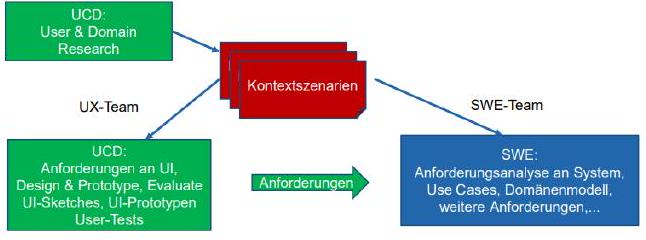
\includegraphics[max width=\textwidth]{2024_12_29_0d1d7b5551ea1b4b41bdg-04(1)}
\end{center}

Abbildung 7: Anforderungsanalyse Übersicht

\subsection*{3.1 Anforderungen aus Artefakten des UCD}
Anforderungen (Requirements): Forderungen bezüglich (Leistungs-) Fähigkeiten oder Eigenschaften die das System unter gegebenen Bedingungen erfüllen muss (explizit oder implizit)

\begin{itemize}
  \item Meist sind nie alle Anforderungen im Voraus vollständig bekannt, entwickeln sich im Laufe des Projekts
  \item Müssen mit den Benutzern und Stakeholdern erarbeitet werden
\end{itemize}

\subsection*{3.2 Anforderungen in Form von Use Cases}
Textuelle Beschreibung einer konkreten Interaktion eines Benutzers mit zukünfigem System (Beschreiben aus Sicht des Akteurs, Impkizite und Explizite Anforderungen, Ziel des Akteurs, Kontext)

\section*{3 Arten von Akteuren}
\begin{itemize}
  \item Primärakteur (Primary Actor)
  \item Initiert einen Anwendungsfall, um sein (Teil-)Ziel zu erreichen\\
Erhălt den Hauptnutzen des Anwendungsfalls\\
Beispiel Kasse: Kassier
  \item Unterstützender Akteur (Supporting Actor)
\end{itemize}

Hilft dem SuD bei der Bearbeitung eines Anwendungsfalls\\
Beispiel Kasse: externer Dienstleister wie Zahlungsdienst für Kreditkarten

\begin{itemize}
  \item Offstage-Akteur (Offstage Actor)
  \item Weitere Stakeholder, die nicht direkt mit dem System interagierten\\
Beispiel Kasse: Steuerbehörde
\end{itemize}

Abbildung 8: Arten von Akteuren

\begin{itemize}
  \item Aus Sicht des Akteurs
  \item Aktiv formuliert (Titel auch aktiv)
  \item Konkreter Nutzen
  \item Mehr als eine einzelne Interaktion / UseCase
  \item im Essentiellen, nicht Konkreten Stil (Logik, nicht Umsetzung)\\
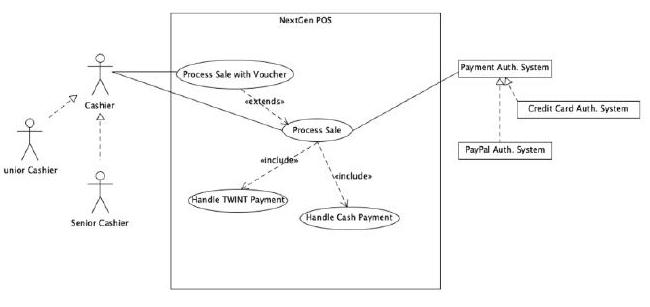
\includegraphics[max width=\textwidth, center]{2024_12_29_0d1d7b5551ea1b4b41bdg-05}
\end{itemize}

Abbildung 9: Use Case Diagramm

\subsection*{3.2.1 Brief UC}
Kurze Beschreibung des Anwendungsfalls in einem Paragraphen

\begin{itemize}
  \item Nur Erfolgsszenario
  \item Sollte enthalten:
  \item Trigger des UCs
  \item Akteure
  \item Summarischen Ablauf des UCs
  \item Wann?: Zu Beginn der Analyse
\end{itemize}

\subsection*{3.2.2 Casual UC}
Informelle Beschreibung des Anwendungsfalls in mehreren Paragraphen

\begin{itemize}
  \item Erfolgsszenario plus wichtigste Alternativszenarien
  \item Sollte enthalten:
  \item Trigger des UCs
  \item Akteure
  \item Interaktion des Akteurs mit System
  \item Wann?: Zu Beginn der Analyse
\end{itemize}

\section*{Formaler Aufbau}
\begin{itemize}
  \item UC-Name
  \item Umfang (Scope)
  \item Ebene (Level)
  \item Primärakteur (Primary Actor)
  \item Stakeholders und Interessen
  \item Vorbedingungen (Preconditions)
  \item Erfolgsgarantie/Nachbedingungen (Success
  \item Erfolgsgarantie/Nachbedingungen (Succe
\end{itemize}

Guarantee)

\begin{itemize}
  \item Standardablauf (Main Sucess Scenario)
  \item Erweiterungen (Extensions)
  \item Spezielle Anforderungen (Special Requirements)
  \item Liste der Technik und Datavariationen\\
(Technology and Data Variations)
  \item Häufigkeit des Auftretens (Frequency of Occurance
  \item Verschiedenes (Miscellaneous)
\end{itemize}

Abbildung 10: Aufbau Fully- Dressed Use Case (UC)

\subsection*{3.2.3 Systemsequenzdiagramm SSD}
Ist formal ein UML Sequenzdiagramm: Zeigt Interaktionen der Akteure mit dem System

\begin{itemize}
  \item Welche Input-Events auf das System einwirken
  \item Welche Output-Events das System erzeugt
\end{itemize}

Ziel:\\
Wichtigste Systemoperationen identifizieren, die das System zur Verfügung stellen muss (API) für einen gegebenen Anwendungsfall

\begin{itemize}
  \item Formal wie Methodenaufruf, evtl mit Parametern, Details zu Parametern sollen im Glossar erklärt werden
  \item Durchgezogener Pfel für Methodenaufruf
  \item Rückgabewert kann fehlen falls unwichtig, indirektes Update des UI, deshalb gestrichelte Linie
\end{itemize}

SSD können auch Interaktionen zwischen SuD und externen unterstützenden System zeigen\\
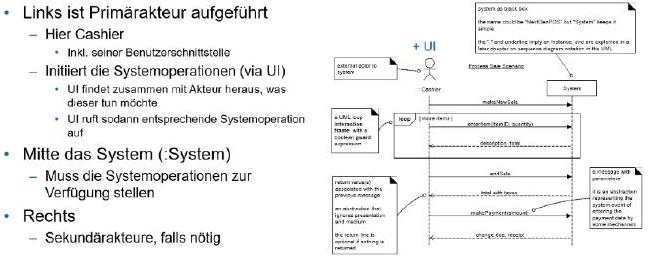
\includegraphics[max width=\textwidth, center]{2024_12_29_0d1d7b5551ea1b4b41bdg-06}

Abbildung 11: Systemsequenzdiagramm (SSD)